% Part 2 chapter carrying "The Cosmological Constant as Actualized Vacuum Energy" (March 2026), sections 1-6, line for line
% (PDF read in full 2026-10-03: 842 text lines, 50-line ledger, no gaps; LaTeX docs/papers/latex/iam_cosmological_constant used
% for exact equation forms). Sections 7-10 are carried in p2_12b_lambda_history.tex. Corrections applied from
% docs/verification/PAPER_ERRATA.md rows C1, C13-C17, C19, C24 and CC_AND_BARYON_CHECK.md items 10-15, 18.
% Not carried (C15, confirmed): the 'holographic round trip 2/pi x pi/2 = 1' and its link to the lepton masses.
% Numbers: docs/verification/scripts/verify_lambda_baryon_book.py (+ _output.txt), sections A, B, D.
\chapter{The cosmological constant}\label{ch:lambda}

The cosmological constant problem is the discrepancy of about 123 orders of magnitude between the vacuum energy density that quantum
field theory gives with a Planck-scale cutoff and the dark-energy density that is observed. It has resisted resolution for over fifty
years. This chapter carries a proposal that the discrepancy arises from a category error: the theoretical vacuum energy density
$\rho_{\rm vac}$ and the observed cosmological constant $\Lambda_{\rm obs}$ are not the same kind of quantity, and within IAM they were
never expected to be equal. \interp

In this reading $\rho_{\rm vac}$ is the complete reservoir of Planck-scale quantum states available on the cosmic horizon: the full set
of states on which records can be written. $\Lambda_{\rm obs}$ is the accumulated Landauer cost of turning Planck-scale vacuum
fluctuations into classical records through irreversible gravitational decoherence on baryonic timelike worldlines over the age of
the universe. The first is a property of the vacuum; the second is a property of the universe's decoherence history. \interp\ The
ratio of the two is then set by the fraction of Planck-area horizon bits that have been written out of the total available, weighted
by the fraction of matter that generates new decoherence events. Only baryons, as decoherence engines on timelike worldlines, are
taken to write new information onto the horizon. \conjecture

The chapter sets out the expression this leads to, evaluates it with Planck 2018 values, and then states what holds and what does not.
What holds is an identity (the 123 orders of magnitude) and one measured relation at the present epoch,
$\Omega_b/\Omega_m=\tfrac3{16}\sqrt{\Omega_\Lambda}$. What comes next is a derivation of the three O(1) factors that turn the
identity into that relation. The history of the accumulation, the growth of $\Lambda$ with time and the conclusions are in
Chapter~\ref{ch:lambda_history}; the baryon density, read through the same relation, is in Chapters~\ref{ch:baryon}
and~\ref{ch:baryon_chain}.

\section{The problem}
The cosmological constant problem is widely regarded as the most significant unsolved problem in theoretical
physics~\cite{Weinberg1989,Martin2012}. Quantum field theory gives a vacuum energy density, from the zero-point fluctuations of all
quantum fields, of the order of the Planck energy density:
\begin{equation}
\rho_{\rm vac}\sim\frac{E_P^4}{(\hbar c)^3}=\frac{c^7}{\hbar G^2}=4.633\times10^{113}\ {\rm J\,m^{-3}},\label{eq:lam_rhovac}
\end{equation}
where $E_P=\sqrt{\hbar c^5/G}=1.956\times10^9$\,J is the Planck energy. \calc\ The observed dark-energy density, inferred from the
accelerating expansion of the universe~\cite{Riess1998,Perlmutter1999}, is
\begin{equation}
\rho_\Lambda=\Omega_\Lambda\rho_cc^2=5.250\times10^{-10}\ {\rm J\,m^{-3}},\qquad \rho_c=\frac{3H_0^2}{8\pi G},\label{eq:lam_rhoL}
\end{equation}
with $H_0=67.4$\,km\,s$^{-1}$\,Mpc$^{-1}$ and $\Omega_\Lambda=0.6846$~\cite{Planck2018VI}. \observed\ The two differ by
\begin{equation}
\frac{\rho_\Lambda}{\rho_{\rm vac}}=1.133\times10^{-123},\qquad \log_{10}\frac{\rho_\Lambda}{\rho_{\rm vac}}=-122.95 .\label{eq:lam_ratio}
\end{equation}
\calc

Proposed resolutions have included supersymmetric cancellation~\cite{Witten2001}, the anthropic selection of vacua from a string
landscape~\cite{BoussoPolchinski2000}, quintessence and dynamical dark energy~\cite{Caldwell1998}, and modifications of
gravity~\cite{Weinberg1989,Carroll2001}. None has achieved broad acceptance. The problem persists because every proposed mechanism
attempts to reduce the theoretical vacuum energy to the observed value: to explain why $\rho_{\rm vac}$ is so small.

The approach carried here is different. The theoretical vacuum energy is not too large, and the observed cosmological constant is not
a fine-tuned residual of a large cancellation. The two quantities are physically distinct and were never expected to be equal. On
this reading the discrepancy is not a consequence of an incorrect theory but of comparing quantities of different physical
character. \interp\ The framework that makes the distinction precise is IAM's Law (Chapter~\ref{ch:iams_law}), in which the
cosmological constant is the accumulated Landauer cost of gravitational decoherence on baryonic timelike worldlines over the age of
the universe, and $\rho_\Lambda/\rho_{\rm vac}$ is a dimensionless geometric quantity: the fraction of Planck-area horizon bits that
baryonic decoherence has written. \conjecture\ Section~\ref{sec:lam_ident} shows that the size of this ratio, $10^{-123}$, follows
from an identity; what a mechanism has to supply is the O(1) factor.

\paragraph{The frame.} IAM's Law: every irreversible transition from a quantum superposition to a classical record pays $k_BT\ln2$ per
bit to the nearest encoding surface, at that surface's temperature, and the record is written on that two-dimensional surface. The
law is the same at every scale at which records are made --- the methylation record of a cell, a switching semiconductor, a measured
qubit, the horizon of a black hole ($T_HS=\tfrac12Mc^2$, Chapter~\ref{ch:blackholes}) --- across some 37 orders of magnitude. At the
cosmic horizon the decoherence is gravitational collapse of matter on timelike worldlines and the surface is the horizon at
$T_{GH}=\hbar H/2\pi k_B$. Nothing here modifies gravity. The Einstein equations are untouched; what is completed is the horizon
entropy functional, the place Jacobson showed the field equations come from~\cite{Jacobson1995}. Jacobson's entropy $S=A/4\ell_P^2$
is purely geometric, and Einstein's $\Lambda$ was a constant he could not identify. Both lack the same piece: $S_{\rm info}$, the
classical information produced by matter decohering on timelike worldlines, encoded on the horizon. Before structure forms
$E(a)\to0$: no structure, no decoherence, no cost, and $\Lambda$ is the vacuum baseline, so the early universe is general relativity
with $\Lambda$, which is $\Lambda$CDM exactly. When matter collapses into halos, galaxies and stars, decoherence accelerates, the
horizon must accommodate the new bits, and the expansion felt by matter speeds up; the structural contribution $S_{\rm info}$,
carried by $\beta_mE(a)$ (Chapter~\ref{ch:theory}), accumulates. The cosmological constant is therefore read as the accumulated
Landauer cost of baryonic decoherence: the baseline before structure, growing with it. Recombination, the acoustic peaks and
nucleosynthesis are unchanged by construction. \conjecture

\section{Two physically distinct quantities}\label{sec:lam_two}
\subsection{The mechanism}
The informational term extends the thermodynamic derivation of the gravitational field equations~\cite{Jacobson1995} by an
informational contribution to the horizon entropy functional. It rests on three established physical principles.
\begin{enumerate}
\item \textbf{Gravitational decoherence on timelike worldlines} is taken as the dominant source of irreversible classical information
production in the universe. Every massive particle that interacts gravitationally decoheres, producing irreversible classical
information at a rate set by the virial theorem (Chapter~\ref{ch:virial}). \interp
\item \textbf{Landauer's principle}~\cite{Landauer1961}: erasing one bit of classical information costs at least $k_BT\ln2$. At the
cosmic horizon temperature $T_H=\hbar H_0/(2\pi k_B)=2.655\times10^{-30}$\,K~\cite{GibbonsHawking1977} each irreversible bit costs
\begin{equation}E_{\rm bit}=\frac{\hbar H_0\ln2}{2\pi}=2.541\times10^{-53}\ {\rm J}.\label{eq:lam_ebit}\end{equation}
\derived\ (the principle) \calc\ (the number)
\item \textbf{The holographic principle}~\cite{tHooft1993,Susskind1995}: irreversible classical information produced by gravitational
decoherence is encoded on the cosmic horizon. The horizon's maximum information content is its Bekenstein--Hawking
entropy~\cite{Bekenstein1973,Hawking1975},
\begin{equation}
N_{\max}=\frac{S}{k_B}=\frac{A_H}{4l_P^2}=\frac{4\pi(c/H_0)^2}{4l_P^2}=2.265\times10^{122}\ \text{nats}=3.268\times10^{122}\ \text{bits},
\label{eq:lam_nmax}\end{equation}
one nat per $4l_P^2$ of horizon and one bit per $4\ln2\,l_P^2$. \derived\ \calc
\end{enumerate}
The result is a single additional Hubble-friction term in the matter-sector perturbation equations --- not a background modification
--- with coupling $\beta_m=\Omega_m/2$, derived from the virial partition (Chapter~\ref{ch:virial}). \derived\ In every chain
(Chapters~\ref{ch:latetime} and~\ref{ch:level2}) $\beta_m$ is held at $\Omega_m/2$, so the chains test the term with $\beta_m$ fixed;
they do not measure $\beta_m$.

\subsection{Two quantities}
Within this reading the theoretical vacuum energy density and the observed cosmological constant are physically distinct. \interp

The vacuum energy density $\rho_{\rm vac}$ is the energy density of the complete Planck-scale quantum substrate: the total zero-point
energy of all quantum fields at all points in space. In the terms of IAM's Law it is the complete reservoir of quantum states
available, at each point of the cosmic horizon, for records to be written on. It is a property of the vacuum itself, independent of
the universe's history. Its natural scale is the Planck energy density because $l_P^2$ sets the area of horizon information: the
Bekenstein--Hawking entropy assigns one nat to each $4l_P^2$ of the cosmic boundary.

The cosmological constant $\Lambda_{\rm obs}$ is the accumulated Landauer cost of turning Planck-scale vacuum fluctuations into
classical records through irreversible gravitational decoherence on baryonic timelike worldlines since the onset of the matter sector
at electroweak symmetry breaking (Chapter~\ref{ch:electroweak}). It is a property of the universe's decoherence history: the running
total of what has been irreversibly written onto the cosmic horizon. Its scale is set by how many Planck-area bits have been written
out of the total horizon-area bits available.

These are not the same quantity. $\rho_{\rm vac}$ is the total available; $\Lambda_{\rm obs}$ is the accumulated written part. Expecting
them to be equal would require the universe to have already turned its entire Planck-scale vacuum energy into classical records --- a
state that corresponds to the asymptotic limit of the activation function, $E(a\to\infty)=e$, which the universe has not reached and
does not reach in finite time. \calc\ (the limit) \interp\ (the reading) The ratio $10^{-123}$ is then the expected ratio of
accumulated record to total capacity in a universe whose decoherence history spans 13.8 billion years but whose total Planck-scale
capacity spans the entire cosmic horizon in Planck units. \interp\ Section~\ref{sec:lam_ident} shows why the size of this number
carries no information beyond $H_0$ in Planck units.

\subsection{The role of dark matter}\label{sec:lam_dm}
A distinction that matters for the writing rate concerns dark matter. In the virial reading of Chapter~\ref{ch:virial_partners}, what
is observed as dark matter is the geometric half of prior gravitational decoherence events: the part of gravitational energy deposited
irreversibly into spacetime curvature at each event. It is therefore already classical geometry, a record already written. It does not
undergo new decoherence events, because decoherence is the passage from a quantum superposition to a classical record, and dark matter
is already on the record side of that passage. \interp

Only baryons --- quantum matter on timelike worldlines that keeps interacting gravitationally and producing new irreversible
information --- drive the ongoing writing rate. The fraction of matter that contributes to the accumulation is then $\Omega_b/\Omega_m$,
not unity. \conjecture\ The order in which the argument runs is: (1) dark matter is read as accumulated geometry
(Chapter~\ref{ch:virial_partners}); (2) so dark matter does not independently decohere; (3) so only baryons contribute to the ongoing
Landauer cost; (4) so the effective writing fraction is $\Omega_b/\Omega_m$; (5) so Eq.~\eqref{eq:base} follows. The factor entered
the expression after comparison with the data, when the residual stood at a factor of 12 (Section~\ref{sec:lam_obj}); until the
coefficient $3/16$ of Section~\ref{sec:lam_rel} is derived, the agreement it produces is \fitted.

\section{The calculation}\label{sec:lam_calc}
\subsection{The ratio}
The fraction of the total vacuum capacity that baryonic gravitational decoherence has written is set by two factors.

First, the geometric factor: the ratio of the Planck area to the total horizon area,
\begin{equation}
f_{\rm geo}=\frac{l_P^2}{A_H}=\frac{l_P^2}{4\pi(c/H_0)^2}=\frac{l_P^2H_0^2}{4\pi c^2}=\frac{1}{4\pi}\left(\frac{l_P}{l_H}\right)^2,
\label{eq:lam_fgeo}\end{equation}
with $l_H=c/H_0$ the Hubble length today. \derived\ (definition)

Second, the baryonic fraction: only baryons write new information onto the horizon, and the fraction of matter that is baryonic is
\begin{equation}f_b=\frac{\Omega_b}{\Omega_m}.\label{eq:lam_fb}\end{equation}
\conjecture\ (that this is the writing fraction)

The expression carried for the ratio of accumulated written part to total capacity is
\begin{equation}
\frac{\rho_\Lambda}{\rho_{\rm vac}}\bigg|_{\rm IAM}=\frac{2}{\pi}\left(\frac{l_P}{l_H}\right)^2\frac{\Omega_b}{\Omega_m}.\label{eq:base}
\end{equation}
The coefficient $2/\pi$ is eight times the $1/4\pi$ of Eq.~\eqref{eq:lam_fgeo}; connecting the two is the next step, and the de Sitter argument offered for it (Section~\ref{sec:lam_twopi}) gives a different number. The coefficient is \openprob.

\subsection{Numerical evaluation}
With Planck 2018 values~\cite{Planck2018VI} and CODATA constants:
\begin{align}
l_P&=\sqrt{\hbar G/c^3}=1.616\times10^{-35}\ {\rm m}, \label{eq:lam_in1}\\
H_0&=67.4\ {\rm km\,s^{-1}\,Mpc^{-1}}=2.184\times10^{-18}\ {\rm s^{-1}}, \label{eq:lam_in2}\\
l_H&=c/H_0=1.373\times10^{26}\ {\rm m}, \label{eq:lam_in3}\\
\Omega_b&=0.0493,\qquad \Omega_m=0.3153 . \label{eq:lam_in4}
\end{align}
\measured\ ($l_P$, $H_0$, $\Omega_b$, $\Omega_m$) \calc\ ($l_H$) The geometric factor and the baryonic fraction are
\begin{equation}
\left(\frac{l_P}{l_H}\right)^2=\left(\frac{1.616\times10^{-35}}{1.373\times10^{26}}\right)^2=1.387\times10^{-122},\qquad
\frac{\Omega_b}{\Omega_m}=\frac{0.0493}{0.3153}=0.1564 .\label{eq:lam_geo}
\end{equation}
\calc\ The expression gives
\begin{equation}
\frac{\rho_\Lambda}{\rho_{\rm vac}}\bigg|_{\rm IAM}=\frac{2}{\pi}\times1.387\times10^{-122}\times0.1564=1.380\times10^{-123},\label{eq:lam_result}
\end{equation}
against the observed ratio from Eqs.~\eqref{eq:lam_rhovac} and~\eqref{eq:lam_rhoL},
\begin{equation}
\frac{\rho_\Lambda}{\rho_{\rm vac}}\bigg|_{\rm obs}=\frac{5.250\times10^{-10}}{4.633\times10^{113}}=1.133\times10^{-123},\label{eq:lam_obs}
\end{equation}
a ratio of prediction to observation of
\begin{equation}
\frac{(\rho_\Lambda/\rho_{\rm vac})_{\rm IAM}}{(\rho_\Lambda/\rho_{\rm vac})_{\rm obs}}=1.218 .\label{eq:lam_factor}
\end{equation}
\calc\ The expression lands within a factor of 1.22 of the observed ratio. It contains the Planck length, the Hubble constant, the
measured density parameters and the coefficient $2/\pi$; Section~\ref{sec:lam_ident} shows that the first two alone fix the
$10^{-123}$.

\subsection{The de Sitter temperature factor}\label{sec:lam_tds}
The factor 1.22 was attributed to the departure from exact de Sitter geometry at the present epoch: dark energy is only 68\,\% of the
energy budget. The Landauer cost per bit is $k_BT\ln2$, with $T$ the temperature of the writing process. Taking that as the
Gibbons--Hawking temperature of the full Hubble rate,
\begin{equation}T_H=\frac{\hbar H_0}{2\pi k_B},\label{eq:lam_TH}\end{equation}
while the encoding surface is the de Sitter horizon, whose temperature is set by the de Sitter rate $H_{dS}=H_0\sqrt{\Omega_\Lambda}$,
\begin{equation}T_{dS}=\frac{\hbar H_{dS}}{2\pi k_B}=T_H\sqrt{\Omega_\Lambda},\label{eq:lam_TdS}\end{equation}
\derived\ (the temperature of the horizon set by $\Lambda$ alone) the cost per bit written on the de Sitter surface is
\begin{equation}E_{\rm bit,eff}=k_BT_{dS}\ln2=k_BT_H\ln2\times\sqrt{\Omega_\Lambda}.\label{eq:lam_Eeff}\end{equation}
Applying the ratio $T_{dS}/T_H=\sqrt{\Omega_\Lambda}$ to Eq.~\eqref{eq:base} gives
\begin{equation}
\frac{\rho_\Lambda}{\rho_{\rm vac}}\bigg|_{T_{dS}}=\frac{2}{\pi}\left(\frac{l_P}{l_H}\right)^2\sqrt{\Omega_\Lambda}\,\frac{\Omega_b}{\Omega_m},
\label{eq:corr}\end{equation}
and with $\Omega_\Lambda=0.6846$,
\begin{equation}
\sqrt{\Omega_\Lambda}=0.8274,\qquad \frac{\rho_\Lambda}{\rho_{\rm vac}}\bigg|_{T_{dS}}=1.380\times10^{-123}\times0.8274=1.142\times10^{-123},
\label{eq:lam_corr_num}\end{equation}
$0.79\,\%$ above the observed value. \calc\ The exponent $p$ of $\Omega_\Lambda$ that would close Eq.~\eqref{eq:base} exactly is
$p=0.521$; $p=\tfrac12$ is the square root of the temperature ratio. \calc\ The factor was applied after the residual of 1.22 had
been seen, and nothing in the derivation fixes beforehand that the writing temperature is $T_H$ and the surface temperature $T_{dS}$
rather than the reverse or the same; until that is fixed, the agreement of Eq.~\eqref{eq:lam_corr_num} is \fitted.

\begin{figure}[htbp]\centering
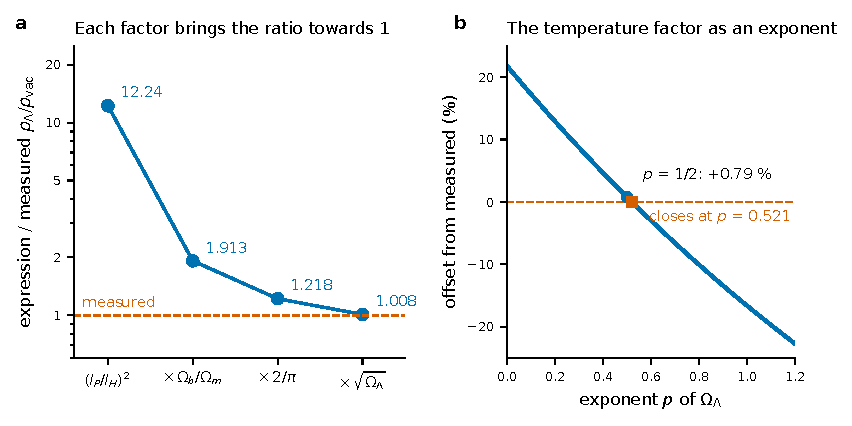
\includegraphics[width=\textwidth]{figures/part2/fig_cc_factors.pdf}
\caption[The factors of the cosmological-constant expression]{The factors of the cosmological-constant expression. (a) The expression divided by the measured $\rho_\Lambda/\rho_{\rm vac}=1.133\times10^{-123}$ as each factor is applied: $(l_P/l_H)^2$ alone is 12.24 times too large, $\Omega_b/\Omega_m$ brings it to 1.913, $2/\pi$ to 1.218 and $\sqrt{\Omega_\Lambda}$ to 1.0079. The identity factor $3\Omega_\Lambda/8\pi$ closes it exactly. (b) $(2/\pi)(l_P/l_H)^2(\Omega_b/\Omega_m)\Omega_\Lambda^p$ against $p$: $p=0.521$ closes it, $p=1/2$ leaves $+0.79\,\%$. Planck 2018 inputs~\cite{Planck2018VI}; CODATA constants. Deriving the three factors is an open problem. \calc\ \openprob}\label{fig:cc_factors}
\end{figure}

\subsection{Summary of the calculation}
Table~\ref{tab:lam_calc} collects the calculation.
\begin{table}[htbp]\centering\small
\caption[The cosmological-constant calculation]{The cosmological-constant calculation. Inputs from Planck 2018~\cite{Planck2018VI} and CODATA; recomputed in \texttt{verify\_lambda\_baryon\_book.py}, section B.}\label{tab:lam_calc}
\begin{tabularx}{\linewidth}{>{\raggedright\arraybackslash}Xlll}\toprule
Quantity & Value & Source & Label\\\midrule
Planck length $l_P$ & $1.616\times10^{-35}$\,m & CODATA & \measured\\
Hubble length $l_H=c/H_0$ & $1.373\times10^{26}$\,m & Planck 2018 $H_0$ & \calc\\
Geometric factor $(l_P/l_H)^2$ & $1.387\times10^{-122}$ & Eq.~\eqref{eq:lam_geo} & \calc\\
Coefficient $2/\pi$ & $0.6366$ & derivation open (Section~\ref{sec:lam_twopi}) & \openprob\\
Baryonic fraction $\Omega_b/\Omega_m$ & $0.1564$ & Planck 2018 & \measured\\
Expression, Eq.~\eqref{eq:base} & $1.380\times10^{-123}$ & Eq.~\eqref{eq:lam_result} & \calc\\
Observed $\rho_\Lambda/\rho_{\rm vac}$ & $1.133\times10^{-123}$ & Eq.~\eqref{eq:lam_obs} & \calc\\
Ratio of the two & $1.218$ & Eq.~\eqref{eq:lam_factor} & \calc\\
With $\sqrt{\Omega_\Lambda}=0.8274$, Eq.~\eqref{eq:corr} & $1.142\times10^{-123}$ ($+0.79\,\%$) & Eq.~\eqref{eq:lam_corr_num} & \fitted\\\bottomrule
\end{tabularx}
\end{table}

\section{The horizon identity}\label{sec:lam_ident}
Writing the critical density in Planck units gives, exactly,
\begin{equation}\frac{\rho_\Lambda}{\rho_{\rm vac}}=\frac{\Omega_\Lambda\,3H_0^2c^2/8\pi G}{c^7/\hbar G^2}
=\frac{3\Omega_\Lambda}{8\pi}\,\frac{\hbar GH_0^2}{c^5}=\frac{3\Omega_\Lambda}{8\pi}\left(\frac{l_P}{l_H}\right)^2,\qquad l_H=c/H_0,\label{eq:ident}\end{equation}
which reproduces $1.133\times10^{-123}$ to all digits. \derived\ The same statement in horizon thermodynamics: the Gibbons--Hawking
temperature~\cite{GibbonsHawking1977} $T_{GH}=\hbar H/2\pi k_B$ times the Bekenstein--Hawking entropy
$S=k_BA/4l_P^2$~\cite{Bekenstein1973,Hawking1975} of the Hubble horizon equals the mass-energy inside it,
\begin{equation}T_{GH}\,S=\frac{\hbar H}{2\pi}\,\frac{\pi c^5}{\hbar GH^2}=\frac{c^5}{2GH}=M_Hc^2\qquad\text{(any }H),\label{eq:lam_smarr}\end{equation}
with $M_H=\rho_c\,\tfrac43\pi(c/H)^3$. \derived\ This is the cosmological counterpart of the Smarr relation of
Chapter~\ref{ch:blackholes}~\cite{Smarr1973}. So $\rho_\Lambda$ is $\Omega_\Lambda$ times the horizon's entropy priced at its own
temperature, per unit Hubble volume. The 123 orders of magnitude are this identity: any expression containing the measured $H_0$ and
the Planck length reproduces them. They are not evidence for a mechanism. What a mechanism must explain is the O(1) factor
$3\Omega_\Lambda/8\pi=0.0817$. \calc\ The derivation is written out step by step, with the status of each premise, in
Appendix~\ref{app:der:lambda}.

\section{What the expression asserts}\label{sec:lam_rel}
\begin{figure}[htbp]\centering
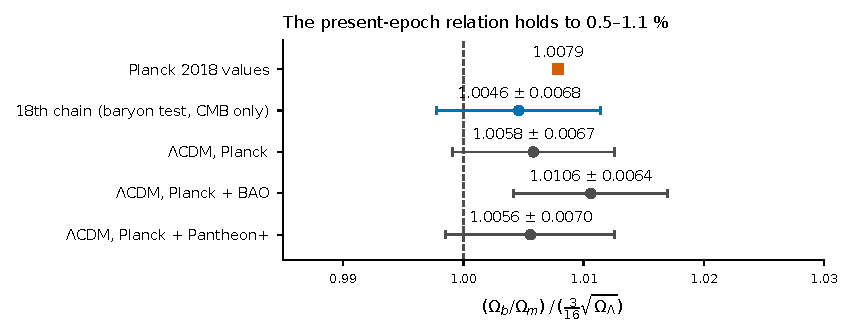
\includegraphics[width=0.75\textwidth]{figures/part2/fig_cc_relation.pdf}
\caption{The present-epoch relation $\Omega_b/\Omega_m=(3/16)\sqrt{\Omega_\Lambda}$, as the ratio of the two sides, on the CMB-only 18th chain ($1.0046\pm0.0068$), on three $\Lambda$CDM chains ($1.0056$--$1.0106$) and on the Planck 2018 values quoted in the text ($1.0079$). Chains: \texttt{mgcamb\_validation/\allowbreak{}chains}, 30\,\% burn-in, weighted (\texttt{verify\_lambda\_baryon\_book.py}, section E). The relation is measured; the derivation of 3/16 is open. \observed\ \openprob}\label{fig:cc_relation}
\end{figure}
Setting Eq.~\eqref{eq:corr} equal to the identity~\eqref{eq:ident}, the $l_P$, $l_H$ and $\pi$ cancel:
\begin{equation}\frac{2}{\pi}\sqrt{\Omega_\Lambda}\,\frac{\Omega_b}{\Omega_m}=\frac{3\Omega_\Lambda}{8\pi}\quad\Longrightarrow\quad
\boxed{\;\frac{\Omega_b}{\Omega_m}=\frac{3}{16}\sqrt{\Omega_\Lambda}\;}\label{eq:rel}\end{equation}
\derived\ (algebra) Without the temperature factor the same step gives $\Omega_b/\Omega_m=3\Omega_\Lambda/16$. \derived\ (algebra)
Planck 2018: $0.1564$ against $0.1551$, a ratio of $1.0079$. \calc\ On the CMB-only 18th chain (Chapter~\ref{ch:baryon_chain}) the
ratio of the two sides is $1.0046\pm0.0068$ ($0.7\sigma$); on the $\Lambda$CDM chains it is $1.0056$--$1.0106$. \measured\ That is
expected: the informational term is off at recombination, so the CMB returns the same $\Omega_b$, $\Omega_m$ and $\Omega_\Lambda$ with
or without it, and the agreement of the chains is a consistency check that the early universe is intact. The relation is a property of
the measured universe; $\Lambda$CDM takes those values as given, and the informational term is what would have to explain them. It
holds at the present epoch only, since $\Omega_\Lambda(a)$ changes and $\Omega_b/\Omega_m$ does not. \observed

Eq.~\eqref{eq:rel} ties the dark-energy fraction to the baryonic fraction of matter. If $3/16$ follows from physics with nothing
adjusted, it explains the O(1) factor that the identity leaves open. \openprob\ How special the agreement is can be measured. Take the
coefficient of $(l_P/l_H)^2$ in the form $q\,\pi^k(\Omega_b/\Omega_m)^i\Omega_\Lambda^j$ with $q$ any of the 23 distinct ratios of
integers from 1 to 6, $k\in\{-1,0,1\}$, $i\in\{0,1\}$ and $j\in\{0,\tfrac12,1\}$: 414 forms. Three land within $1\,\%$ of the measured
$0.0817$, among them Eq.~\eqref{eq:corr} ($0.7\,\%$ of the forms). \calc\ So the derivation, not the agreement, carries the weight.
The algebra and every factor are set out in Appendix~\ref{app:der:lambda}.

\section{The Planck cutoff}\label{sec:lam_cutoff}
The calculation depends on the ultraviolet cutoff of the vacuum energy. With a cutoff at mass scale $M$,
$\rho_{\rm vac}(M)=M^4/(\hbar c)^3$, and the observed ratio grows by $(E_P/M)^4$: $2.2\times10^{68}$ for an electroweak cutoff
(100\,GeV) and $1.4\times10^{79}$ for a QCD cutoff (200\,MeV), so that $\rho_\Lambda/\rho_{\rm vac}$ would be $2.5\times10^{-55}$ and
$1.6\times10^{-44}$, and an expression in $(l_P/l_H)^2$ no longer applies. \calc\ The choice needs a reason.

Within IAM's Law the Planck cutoff is not an arbitrary regularization; it is set by the horizon encoding. The Bekenstein--Hawking
entropy~\cite{Bekenstein1973,Hawking1975}, $S=A/(4l_P^2)$, gives the area per unit of horizon information: one nat per $4l_P^2$, one
bit per $4\ln2\,l_P^2$. The vacuum energy computed at the Planck cutoff is then the energy density associated with the complete set of
Planck-area information states available on the horizon --- one quantum of capacity per quantum of encodable area. Any lower cutoff
would count only part of the available states. The Planck scale is the natural cutoff not as a regularization convenience but as the
scale at which the vacuum capacity and the horizon encoding capacity are commensurate. \interp

The argument does not apply at lower cutoffs. The electroweak and QCD scales are thresholds for specific field contributions to the
vacuum energy, but they are not the fundamental quantum of horizon information. The Planck area is the irreducible unit of boundary
encoding, and the vacuum energy at the Planck cutoff is the quantity commensurate with it. \interp\ In the relation~\eqref{eq:rel}
the cutoff cancels; it fixes only how the result is written.

\section{The coefficient $2/\pi$ and the de Sitter causal structure}\label{sec:lam_twopi}
The expression~\eqref{eq:base} includes the coefficient $2/\pi$, which needs a physical reason. The place to look is the causal
structure of de Sitter space, the geometry of a universe with positive cosmological constant, which describes the universe at late
times.

\subsection{The horizon of a de Sitter observer}
In de Sitter space the cosmological horizon is observer-dependent. Every observer is surrounded by a causal horizon that divides the
universe into the static patch, causally accessible to the observer, and the region beyond the horizon, causally inaccessible. One
route takes the static patch to subtend $2\pi$ of the horizon's $4\pi$\,sr, by analogy with the Rindler horizon, which
separates the half of Minkowski spacetime from which a uniformly accelerated observer can receive signals. That analogy concerns
regions of spacetime, not solid angle. The static patch of a de Sitter observer is bounded by the whole horizon sphere, and the
observer receives signals from all $4\pi$\,sr of it. \derived

\subsection{Consequence for the accumulation}
On the argument offered, the observer's decoherence events write only on the causally accessible part of the horizon, information
written beyond the horizon cannot contribute to the observable cosmological constant, and the effective writing area is
\begin{equation}A_{\rm eff}=\tfrac12\times4\pi l_H^2=2\pi l_H^2 .\label{eq:lam_aeff}\end{equation}
The number of Bekenstein--Hawking units in that area is
\begin{equation}N_{\rm eff}=\frac{A_{\rm eff}}{4l_P^2}=\frac{2\pi l_H^2}{4l_P^2}=\frac{\pi l_H^2}{2l_P^2}\ \text{nats},\label{eq:lam_nbits}\end{equation}
\derived\ (arithmetic) and the fraction of vacuum energy per accessible unit, in the form offered, is
\begin{equation}f_{\rm bit}=\frac{l_P^2}{A_{\rm eff}/(4\pi)}=\frac{4\pi l_P^2}{2\pi l_H^2}=2\left(\frac{l_P}{l_H}\right)^2 .\label{eq:lam_fbit}\end{equation}
\derived\ (arithmetic) The area $A_{\rm eff}=2\pi l_H^2$ gives $2(l_P/l_H)^2$, not $(2/\pi)(l_P/l_H)^2$; with the full horizon area it
gives $(l_P/l_H)^2$. Neither the geometric factor~\eqref{eq:lam_fgeo} nor the de Sitter argument yields $2/\pi$, and the argument's premise (half the horizon) does not hold. Deriving the coefficient $2/\pi$ is the open problem. \openprob

\subsection{Departure from exact de Sitter}
The argument was meant to apply in the de Sitter limit, where dark energy dominates the energy budget entirely. Today dark energy is
about 68\,\% of the total energy density and matter about 32\,\%, so exact de Sitter is an approximation at the present epoch. The
temperature factor $T_{dS}/T_H=\sqrt{\Omega_\Lambda}=0.8274$ of Section~\ref{sec:lam_tds} was introduced for that departure. The full cosmic decoherence history integral (Chapter~\ref{ch:lambda_history}) is meant to give a second derivation of the same factor from the epoch-dependent accumulation; as written it does not converge, and making it converge is the next step. \openprob

\section{Three objections}\label{sec:lam_obj}
Three objections are most likely to be directed at the expression. Each is stated with the response IAM's Law gives and what the
recomputation shows.

\subsection{The Planck cutoff is arbitrary}
\emph{Objection.} The vacuum energy calculation is sensitive to the ultraviolet cutoff. The Planck cutoff is not uniquely determined by
established physics, and other cutoffs give completely different results. The agreement within a factor of 1.2 is therefore
cutoff-dependent and not a robust prediction.

\emph{Response.} Within IAM's Law the Planck cutoff is physically set, not arbitrary. The question is what fraction of the complete
Planck-scale vacuum capacity baryonic decoherence has written into records. The natural unit for that fraction is the ratio of one
Planck-area unit to the total horizon area in Planck units. The Bekenstein--Hawking entropy makes $l_P^2$ (times 4, or $4\ln2$ per bit)
the area per unit of horizon information; it is the quantum of the encoding surface. Computing the vacuum energy at any lower cutoff
would undercount the available states and give an incoherent ratio. \interp\ The argument is specific to IAM's Law and does not apply
to standard quantum-field-theory vacuum calculations, where the Planck cutoff is a regularization choice. Eq.~\eqref{eq:base} is
therefore a conditional result: it holds if the vacuum energy is the Planck-scale capacity of the horizon encoding substrate. In the
relation~\eqref{eq:rel} the cutoff cancels (Section~\ref{sec:lam_cutoff}).

\subsection{The factor $\Omega_b/\Omega_m$ was introduced to improve agreement}
\emph{Objection.} The factor $\Omega_b/\Omega_m$ appears to have been introduced to reduce the discrepancy from a factor of 12 to a
factor of 1.2. That is parameter fitting, not prediction.

\emph{Response.} The factor is not a free parameter: it is a measured ratio, and the physical argument for it is the reading of dark
matter as accumulated geometry (Section~\ref{sec:lam_dm}). In that reading dark matter is spacetime curvature laid down by the
gravitational energy of decoherence; it is already classical geometry and does not undergo new quantum decoherence events. Only
baryons --- matter that continues to exist in quantum superposition and to interact gravitationally, producing new irreversible
information --- write new bits onto the horizon. \interp

\emph{What the record shows.} The factor entered the expression after comparison with the data: without it the expression is
$12.24$ times the observed ratio, with it $1.913$, and with $2/\pi$ then $1.218$ (Fig.~\ref{fig:cc_factors}a). \calc\ The physical
argument is the reason given for the factor; the sequence in which the factors were applied means the agreement they produce is
\fitted\ until the coefficient $3/16$ is derived.

\subsection{The remaining factor of 1.2 indicates an incomplete theory}
\emph{Objection.} A factor of 1.2 means the calculation is not exact. Without an explanation for it, the agreement may be
coincidental rather than physical.

\emph{Response.} The factor was attributed to the departure from exact de Sitter geometry: the Gibbons--Hawking temperature of the de
Sitter encoding surface, $T_{dS}=T_H\sqrt{\Omega_\Lambda}$, differs from the writing temperature $T_H$ by $\sqrt{\Omega_\Lambda}=0.8274$,
and applying it (Eq.~\eqref{eq:corr}) gives $1.142\times10^{-123}$ against $1.133\times10^{-123}$. The square root follows from the
ratio of temperatures, which are linear in $H$, while $\Omega_\Lambda$ is quadratic in $H$. \derived

\emph{What the recomputation shows.} (1) The exponent that closes Eq.~\eqref{eq:base} exactly is $0.521$, and $p=\tfrac12$ leaves
$+0.79\,\%$. \calc\ (2) The $10^{-123}$ is the identity~\eqref{eq:ident}: any O(1) prefactor of $(l_P/l_H)^2$ lands within a factor
of a few of the observed ratio, so recovering it ``within a factor of 2'' from the Planck length and the Hubble constant is guaranteed,
not improbable. The meaningful count is the one in Section~\ref{sec:lam_rel}: 3 of 414 O(1) forms within $1\,\%$. \calc\ (3) The
problem as stated spans 123 orders of magnitude; Eq.~\eqref{eq:base} is within a factor of 1.22 and Eq.~\eqref{eq:corr} within
$0.79\,\%$, but the 123 orders are carried by the identity, and deriving the remaining O(1) factors is an open problem. \openprob

The identity carries the orders of magnitude; what remains is a set of concrete factors, each stated with its status. A cosmologist or a particle theorist can take any one of them and try to derive it, or break it.

\section{Status}
Stands: the identity~\eqref{eq:ident} and $T_{GH}S=M_Hc^2$ \derived; the measured relation~\eqref{eq:rel} at the present epoch
(0.5--1.1\,\% on every chain) \observed. Open: a derivation of $3/16$ in which the geometric factor, the temperature factor and the
baryon fraction each follow from physics, which must also explain why the relation holds now. \openprob\ Unaffected: general
relativity with the informational term, which is $\Lambda$CDM before structure and differs only in late-time growth
(Chapters~\ref{ch:latetime}--\ref{ch:level2}). The growth of $\Lambda$ with time, the history integral and the conclusions follow in
Chapter~\ref{ch:lambda_history}.
\begin{table}[htbp]\centering\small
\caption[The cosmological-constant numbers]{The cosmological-constant numbers of this chapter and Chapter~\ref{ch:lambda_history} (Planck 2018: $H_0=67.4$, $\Omega_b=0.0493$, $\Omega_m=0.3153$, $\Omega_\Lambda=0.6846$; chains with 30\,\% burn-in, weighted). Recomputed with \texttt{docs/verification/scripts/\allowbreak{}verify\_lambda\_baryon\_book.py}.}\label{tab:lambda_numbers}
\begin{tabularx}{\linewidth}{>{\raggedright\arraybackslash}Xll}\toprule
Quantity & Value & Label\\\midrule
$\rho_{\rm vac}=E_P^4/(\hbar c)^3$ & $4.633\times10^{113}$\,J\,m$^{-3}$ & \calc\\
$\rho_\Lambda=\Omega_\Lambda\rho_cc^2$ & $5.250\times10^{-10}$\,J\,m$^{-3}$ & \observed\\
$\rho_\Lambda/\rho_{\rm vac}$, and the identity $(3\Omega_\Lambda/8\pi)(l_P/l_H)^2$ & $1.133\times10^{-123}$ (both) & \derived\\
Horizon capacity $A_H/4l_P^2$ today & $2.265\times10^{122}$ nats ($3.268\times10^{122}$ bits) & \calc\\
$(2/\pi)(l_P/l_H)^2\,\Omega_b/\Omega_m$ & $1.380\times10^{-123}$ ($\times1.218$) & \calc\\
$\times\sqrt{\Omega_\Lambda}$ & $1.142\times10^{-123}$ ($+0.79\,\%$) & \fitted\\
Exponent $p$ of $\Omega_\Lambda$ that closes the expression & $0.521$ & \calc\\
$\Omega_b/\Omega_m$ against $(3/16)\sqrt{\Omega_\Lambda}$, Planck values & $0.1564$ against $0.1551$ & \observed\\
Ratio of the two sides, 18th chain (CMB only) & $1.0046\pm0.0068$ & \measured\\
Ratio of the two sides, $\Lambda$CDM chains & $1.0056$--$1.0106$ & \measured\\
O(1) forms within $1\,\%$ of $3\Omega_\Lambda/8\pi$ & 3 of 414 & \calc\\
History integral as written, coefficient against the required $0.523$ & $3.1\times10^{30}$ & \calc\\
Heat radiated by baryonic virialisation, summed to today, over $\rho_\Lambda c^2$ & $3.15\times10^{-8}$ & \calc\\
A derivation of $3/16$ from physics & --- & \openprob\\\bottomrule
\end{tabularx}
\end{table}
